\usetikzlibrary{decorations.fractals}
%--------------------------------------------------------------------------
\tikzset{
    disc/.style={shade, shading=radial, 
                 rounded rectangle,
                 minimum height=.5cm,
                 inner color=#1!20, 
                 outer color=#1!60!gray},
    disc 1/.style={disc=yellow, minimum width=15mm},
    disc 2/.style={disc=orange, minimum width=20mm},
    disc 3/.style={disc=red, minimum width=25mm},
    disc 4/.style={disc=green, minimum width=30mm},
    disc 5/.style={disc=blue, minimum width=35mm},
    disc 6/.style={disc=purple, minimum width=40mm},
}
%--------------------------------------------------------------------------
\def\pole{
  \fill[gray] (-1.6, 0) rectangle (1.6,0.25)
              (-0.125,0.25) rectangle (0.125,3.30);}
%--------------------------------------------------------------------------
%--------------------------------------------------------------------------
%--------------------------------------------------------------------------
\chapter{Récursivité}
%--------------------------------------------------------------------------
%--------------------------------------------------------------------------
%--------------------------------------------------------------------------
\begin{center}
{\huge\bf GNU : GNU's Not UNIX} 
\end{center}

\begin{abstract}
    Dans ce chapitre nous allons définir un nouveau moyen de faire des calculs répétitifs : on appellera la fonction dans sa définition. C'est un outil très puissant qui permettra d'écrire simplement des algorithmes difficiles. La contrepartie est qu'il faudra gérer avec soin les conditions de terminaison.
    
Une fonction est {\bf récursive} si, dans sa définition, elle fait référence à elle-même. 
Les fonctions non récursives seront dites {\bf itératives}.

Une notion importante sera celle de {\bf condition d'arrêt}.
\end{abstract}
%--------------------------------------------------------------------------
%--------------------------------------------------------------------------
\section{Exemples}
%--------------------------------------------------------------------------
%--------------------------------------------------------------------------
\subsection{Factorielle}
%--------------------------------------------------------------------------
%--------------------------------------------------------------------------
La factorielle de $n$, $n!$, est définie par $n!=\prod\limits_{k=1}^n k$ avec la convention $0!=1$.
On peut traduire cette définition par une définition par récurrence :
$\displaystyle n!= \left\{\begin{matrix} 1 & \hbox{si }n=0 \cr  n. (n-1)!&\hbox{sinon}\cr \end{matrix}\right.$.

Cela donne immédiatement l'algorithme
%--------------------------------------------------------------------------
\begin{lstlisting}
def factoriel(n):
  """Entrée : un entier positif n
     Sortie : la factorielle de n"""
    if n==0 :
        return 1
    else :
        return n*factoriel(n-1)
\end{lstlisting}
%--------------------------------------------------------------------------

Que fait la machine lors de l'appel \type{factoriel(3)} ?
%--------------------------------------------------------------------------
\begin{itemize}
\item Elle stocke la formule \type{3*factoriel(2)}.

\item L'appel \type{factoriel(2)} remplace \type{factoriel(2)} par \type{2*factoriel(1)}.

\item L'appel \type{factoriel(1)} remplace \type{factoriel(1)} par \type{1*factoriel(0)}.

\item L'appel \type{factoriel(0)}  retourne 1 ce qui permet de calculer $1*1$ pour \type{factoriel(1)}

\item Les calcul stockés donnent alors $2*1$ pour \type{factoriel(2)} puis $3*2$ pour \type{factoriel(3)}.

\end{itemize}
%--------------------------------------------------------------------------
Sur cet exemple, on voit que la machine doit stocker en mémoire un ensemble de formules. Nous verrons dans la suite la structure de \Type{pile} qui représente ce stockage. 

L'appel à \type{factoriel(0)} signe la fin de la construction de cette pile. Ensuite  elle est parcourue en sens inverse pour permettre les calculs numériques. On comprend l’étymologie du mot récursivité qui vient de {\it recurrere} en latin qui signifie {\it revenir en arrière}.

S'il n'existait pas de condition d'arrêt l'empilement continuerait sans fin, il y aurait saturation de la mémoire : on parle de {\it stack overflow} en anglais. Dans la pratique Python bloque la pile à une longueur de 1000.
%-------------------------------------------------------------------------------%--------------------------------------------------------------------------
\subsection{Tours de Hanoï}
%--------------------------------------------------------------------------
%--------------------------------------------------------------------------
Le problème des tours de Hanoï est un jeu de réflexion imaginé par le mathématicien français Édouard Lucas consistant à déplacer des disques de diamètres différents d'une tour de ``départ'' à  une tour d'``arrivée'' en passant par une tour ``intermédiaire'' tout en respectant les règles suivantes :
%--------------------------------------------------------------------------
\begin{itemize}
\item on ne peut déplacer plus d'un disque à la fois,
\item on ne peut placer un disque que sur un autre disque plus grand que lui ou sur un emplacement vide.
\end{itemize}
%--------------------------------------------------------------------------
Au départ les disques sont placés en respectant la seconde règle sur la tout de départ.

On part de :
%%--------------------------------------------------------------------------
\[
\begin{tikzpicture}
  \foreach \x in {0cm,3.8cm,7.6cm} {\startscope[xshift=\x] \pole \stopscope};
  \node[disc 5,yshift=0.5cm]{5};
  \node[disc 4,yshift=1.0cm]{4};
  \node[disc 3,yshift=1.5cm]{3};
  \node[disc 2,yshift=2.0cm]{2};
  \node[disc 1,yshift=2.5cm]{1};
\end{tikzpicture}
\]
%--------------------------------------------------------------------------
On veut arriver à
%--------------------------------------------------------------------------
\[
\begin{tikzpicture}
  \foreach \x in {0cm,3.8cm,7.6cm} {\startscope[xshift=\x] \pole \stopscope};
  \startscope[xshift=7.6cm]
    \node[disc 5,yshift=0.5cm]{5};
    \node[disc 4,yshift=1.0cm]{4};
    \node[disc 3,yshift=1.5cm]{3};
    \node[disc 2,yshift=2.0cm]{2};
    \node[disc 1,yshift=2.5cm]{1};\stopscope
\end{tikzpicture}
\]
%--------------------------------------------------------------------------
Une position intermédiaire possible serait
%--------------------------------------------------------------------------
\[
\begin{tikzpicture}
  \foreach \x in {0cm,3.8cm,7.6cm} {\startscope[xshift=\x] \pole \stopscope};
  \node[disc 1,yshift=0.5cm]{1};
  \startscope[xshift=3.8cm]
    \node[disc 4,yshift=0.5cm]{4};
    \node[disc 3,yshift=1.0cm]{3};\stopscope
  \startscope[xshift=7.6cm]
    \node[disc 5,yshift=0.5cm]{5};
    \node[disc 2,yshift=1.0cm]{2};\stopscope
\end{tikzpicture}
\]
%--------------------------------------------------------------------------
Dans cette dernière position il y a 3 déplacements possibles :
%--------------------------------------------------------------------------
\begin{itemize}
  \item déplacer le disque 1 au-dessus du disque 3,
  \item déplacer le disque 1 au-dessus du disque 2,
  \item déplacer le disque 2 au-dessus du disque 3.
\end{itemize}
%--------------------------------------------------------------------------
La résolution est en fait simple à énoncer en renonçant à écrire la stratégie de manière précise : pour déplacer $n$ disques de la tour A la tour B il suffit 
%--------------------------------------------------------------------------
\begin{itemize}
  \item de ne rien faire si $n=0$

\item de déplacer les $n-1$ disques supérieurs de la tour A vers la tour C,

 puis de déplacer le disque restant vers la tour B
 
 puis enfin  de déplacer les $n-1$ disques supérieurs de la tour C vers la tour B.
\end{itemize}
%--------------------------------------------------------------------------
On voit apparaître naturellement un algorithme récursif.
%--------------------------------------------------------------------------
\begin{lstlisting}
def hanoi(n,ch1,ch2,ch3):
    """Entrée : un entier et 3 noms de tours
       Sortie : les mouvements à faire pour déplacer 
                les disques depuis la tour nommée ch1 
                vers la tour nommée ch2"""
    if n != 0:
        hanoi(n-1,ch1,ch3,ch2)
        print('Déplacer le disque supérieur de {} vers {}'.format(ch1,ch2))
        hanoi(n-1,ch3,ch2,ch1)  
\end{lstlisting}
%--------------------------------------------------------------------------
On obtient alors un mode d'emploi.
%--------------------------------------------------------------------------
\begin{lstlisting}
Déplacer le disque supérieur de A vers C
Déplacer le disque supérieur de A vers B
Déplacer le disque supérieur de C vers B
Déplacer le disque supérieur de A vers C
Déplacer le disque supérieur de B vers A
Déplacer le disque supérieur de B vers C
Déplacer le disque supérieur de A vers C
Déplacer le disque supérieur de A vers B
Déplacer le disque supérieur de C vers B
Déplacer le disque supérieur de C vers A
Déplacer le disque supérieur de B vers A
Déplacer le disque supérieur de C vers B
Déplacer le disque supérieur de A vers C
Déplacer le disque supérieur de A vers B
Déplacer le disque supérieur de C vers B
\end{lstlisting}
%--------------------------------------------------------------------------
On voit ici le caractère un peu magique de la récursivité : on dit très simplement les choses et le programme produit un résultat compliqué.
Contrairement à l'exemple suivant, la récursivité ici est tout-à-fait naturelle ; il est difficile d'écrire un programme non récursif.
%--------------------------------------------------------------------------
\subsubsection{Complexité}
%--------------------------------------------------------------------------

On va estimer la complexité en comptant le nombre, noté $C(n)$, d'instructions \type{print} que le programme effectue, on note $C(n)$.
Ici encore on va avoir une récurrence. 

Si $n=0$ on a $C(0)=0$. 

Quand on appelle la fonction pour $n$ disques on effectue
%--------------------------------------------------------------------------
\begin{itemize}
  \item $C(n-1)$ instructions \type{print} dans \type{hanoi(n-1,ch1,ch3,ch2)}
  
  \item 1 instruction \type{print} dans \type{print('Déplacer le disque supérieur de',ch1,'vers',ch2)}

  \item $C(n-1)$ instructions \type{print} dans \type{hanoi(n-1,ch3,ch2,ch1)}.
  
  \item On a donc $C(n)=2C(n-1)+1$ pour $n\ge 1$.
\end{itemize}
%--------------------------------------------------------------------------
$\bigl(C(n)\bigr)$ vérifie donc une relation arithmético-géométrique. 

Le point fixe est $-1$ donc $u_n=C(n)-(-1)$ vérifie $u_n=2u_{n-1}$ avec $u_0=C(0)+1=1$ d'où $u_n=2^n$ puis $C(n)=2^n-1$.
Nos 5 petites lignes de code ont créé un monstre de complexité !
%--------------------------------------------------------------------------
%--------------------------------------------------------------------------
\subsection{Transformation d'un programme}
%--------------------------------------------------------------------------
%--------------------------------------------------------------------------
Considérons le programme classique de calcul de la somme des termes d'une liste
%--------------------------------------------------------------------------
\begin{lstlisting}
def somme(liste):
    """Entrée : une liste de nombres
       Sortie : la somme des termes de la liste"""
    resultat = 0
    n = len(liste)
    for i in range(n):
        resultat = resultat + liste[i]
    return resultat
\end{lstlisting}
%--------------------------------------------------------------------------
On a défini un invariant de boucle : à chaque valeur de $i$ au début de la boucle \type{resultat} vaut la somme de $i$ premiers termes. En fait cet invariant définit la somme par récurrence avec, comme toutes les récurrences, 2 assertions.

\begin{description}
  \item[Comment initialiser ?] Ici une somme de 0 termes vaut 0.
  \item[Comment avancer ?] $\displaystyle \sum_{k=0}^i u_k = u_i + \sum_{k=0}^{i-1} u_k$.
\end{description} 
  
\medskip

La récursivité consiste à traduire ces propriétés en un algorithme : 
%--------------------------------------------------------------------------
\begin{itemize}
  \item une somme vide vaut 0,

\item la somme de $n$ termes d'une liste est l'addition du dernier terme à la somme des $n-1$ premiers.
\end{itemize}
%--------------------------------------------------------------------------
\begin{lstlisting}
def somme(liste):
    """Entrée : une liste de nombres
       Sortie : la somme des termes de la liste"""
    n = len(liste)
    if n == 0:
        return 0
    else:
        return  liste[n-1] + somme(liste[:n-1])
\end{lstlisting}
%-------------------------------------------------------------------------------
{\bf Remarque} : dans le programme ci-dessus on fait bien $n$ additions pour calculer une somme : on n'a pas compliqué le calcul.
Cependant à chaque appel on invoque \type{liste[:n-1]} qui effectue une copie de la liste, cela demande $n-1$ opérations de copie de valeurs. Quand on fait le bilan on arrive à $\frac {n(n-1)}2$ copies. Ce temps de recopie finit par surpasser le temps de calcul des sommes et le programme sera lent pour des grandes valeurs de $n$.

Cette difficulté doit inciter à la prudence : il est inutile d'écrire une fonction récursive si on sait écrire une fonction simplement sans récursivité.
%--------------------------------------------------------------------------
%--------------------------------------------------------------------------
\section{Analyse des algorithmes récursifs}
%--------------------------------------------------------------------------
%--------------------------------------------------------------------------
\subsection{Emploi de récurrences}
%--------------------------------------------------------------------------
L'outil principal qui est utilisé dans l'analyse de fonctions récursive est la récurrence.
%--------------------------------------------------------------------------
\subsection{Terminaison}
%--------------------------------------------------------------------------
 L'expérience montre qu'il est très facile d'écrire un algorithme récursif qui ne termine pas. En effet il peut se produire que la fonction fasse indéfiniment appel à elle même. Un cas caricatural est la fonction suivante.
%--------------------------------------------------------------------------
\begin{lstlisting}
def f(x):
  return f(x+1)
\end{lstlisting}
%--------------------------------------------------------------------------
Pour qu'un algorithme récursif termine il est donc indispensable qu'il existe une {\bf condition d'arrêt}, c'est-à-dire une condition qui, si elle est réalisée, fait exécuter des instructions qui ne font pas appel (récursivement) à la fonction. Il est recommandé de commencer par ce cas dans la rédaction de l'algorithme.

Il faut de plus que l'on soit certain que toute suite d'appels à la fonction finit par aboutir à un cas où cette condition est vérifiée.

On pourra souvent mettre en évidence un paramètre (ou d'une expression des paramètres) qui ne prend que des valeurs entières positives. La preuve de la terminaison se fera alors par récurrence sur ce paramètre. 
%--------------------------------------------------------------------------
\subsection{Correction}
%--------------------------------------------------------------------------

Les algorithmes récursifs sont souvent bien adaptés pour être prouvés par récurrence. Parfois même ils sont la traduction d'une définition récursive qui en fournit alors directement la preuve.
%--------------------------------------------------------------------------
\subsection{Complexité}
%--------------------------------------------------------------------------
La complexité vérifiera souvent une relation de récurrence, parfois sous la forme d'une inégalité. Ici encore on aura souvent besoin de faire une démonstration par récurrence.
%--------------------------------------------------------------------------
\section{Exemples}
%--------------------------------------------------------------------------
\subsection{Factorielle}
%--------------------------------------------------------------------------
  On montre par récurrence sur $n$ la propriété ${\cal P}(n)$ : 
  
  pour tout $n$ la fonction renvoie $n!$ en effectuant $n$ multiplications.
 %--------------------------------------------------------------------------
\subsection{Tours de Hanoï}
%--------------------------------------------------------------------------
   On montre par récurrence sur $n$ la propriété ${\cal P}(n)$ : 
    pour tout liste de taille $n$ la fonction affiche les instructions qui permettent de déplacer $n$ disques en respectant les règles.
  
  La complexité a été calculée, par récurrence.
%--------------------------------------------------------------------------
\subsection{Somme des termes d'une liste}
%--------------------------------------------------------------------------
  On montre par récurrence sur $n$ la propriété ${\cal P}(n)$ : 
    pour tout liste de taille $n$ la fonction renvoie la somme des termes de la liste en effectuant $n$ additions.
%--------------------------------------------------------------------------
\subsection{Coefficients binomiaux}
%--------------------------------------------------------------------------
Pour $0\le p\le n$, $\displaystyle \binom n p=\frac{n!}{p!(n-p)!}$.

Un résultat mathématique classique est que $\displaystyle \binom n p=\frac np.\binom n p{n-1}{p-1}$ pour $p\ge 1$.

En ajoutant la condition d'arrêt pour $p=0$, $\binom n 0= 1$, on obtient l'algorithme
%--------------------------------------------------------------------------
\begin{lstlisting}
def binomial(n,p):
  """Entrée : deux entiers positifs
     Requis : 0 <= p <= n
     Sortie : p parmi n"""
    if p == 0:
        return 1
    else :
        return n*binomial(n-1,p-1)//p
\end{lstlisting}
%--------------------------------------------------------------------------
On peut remarquer que l'on ne fait que des calculs sur les entiers.
%--------------------------------------------------------------------------
\begin{itemize}
  \item Le programme renvoie un résultat pour $p=0$ et pour tout $n$.
  
  S'il renvoie un résultat pour $p$ et pour tout $n$ tel que $n\ge p$ alors \type{binomial(n, p+1)} avec $n\ge p+1$ fait appel à \type{binomial(n - 1, p)} qui fournit un résultat ($n-1 \ge p$) et effectue 2 opérations pour renvoyer un résultat
  
  Par récurrence sur $p$ on voit que le programme renvoie un résultat pour tout $p$ et pour tout $n\ge p$.
  \item Le programme renvoie 1 pour $p=0$ et on a bien $\binom n0=1$
  
  Si \type{binom(n p)} renvoie $\binom np$ pour tout $n\ge p$ alors  \type{binomial(n, p+1)} avec $n\ge p+1$ renvoie $\frac n{p+1}.\binom{n-1}p = \binom n{p+1}$.
  
  Par récurrence sur $p$ on voit que le programme renvoie $\binom np$ pour tous $n\ge p$.
  \item On a vu que \type{binomial(n, p)} effectuait 2 opérations de plus que  \type{binomial(n-1, p-1)} donc $2p$ opérations de plus que  \type{binomial(n-p, 0)} : la complexité est $2p$.
  
  \end{itemize}
%-------------------------------------------------------------------------------
\subsection{Recherche par dichotomie}
%--------------------------------------------------------------------------
On suppose qu'on a une liste triée (d'entiers par exemple).

On veut savoir si un élément appartient à la liste.

Pour cela on teste au milieu de la liste :
%--------------------------------------------------------------------------
\begin{itemize}
\item si on a trouvé, c'est fini,
\item si la valeur au milieu est inférieure à la valeur recherchée alors on doit chercher dans la partie supérieure,
\item sinon on doit chercher dans la partie inférieure.
\end{itemize}
%--------------------------------------------------------------------------
L'algorithme est naturellement récursif si on considère une fonction qui recherche un élément dans une liste entre deux positions.
%--------------------------------------------------------------------------
\begin{lstlisting}
def chercher_entre(x, liste, debut, fin):
    """Entrées : un nombre x, une liste de nombres, 2 indices
       Requis  : la liste est triée
                 0 <= debut, fin < len(liste)
       Sortie  : True ou False selon que x aparaît ou non 
                 dans la liste entre debut et fin"""
    if debut > fin: # On ne peut plus chercher 
        return False
    else:
        m = (debut + fin)//2 
        if liste[m] == x:
            return True    
        elif liste[m] < x: 
            return chercher_entre(x, liste, m+1, fin) 
        else: 
            return chercher_entre(x, liste, debut, m-1)
\end{lstlisting}
%--------------------------------------------------------------------------
On peut alors en déduire une fonction de recherche dans une liste triée.
%--------------------------------------------------------------------------
\begin{lstlisting}
def appartient(x, liste):
    n = len(liste)
    return chercher_entre(x, liste, 0, n-1)  # on cherche partout
\end{lstlisting}
%-------------------------------------------------------------------------------
\subsubsection{Terminaison}
%--------------------------------------------------------------------------
Pour prouver que la fonction \type{chercher\_entre} termine on note $k$ la valeur de \type{fin - debut} et on procède par récurrence généralisée sur $k$.

Pour $k < 0$ l'algorithme fournit le résultat \type{False}.
  
On suppose que l'algorithme fournit un résultat pour tout $k < k_0$.
  
  Si \type{fin - debut} vaut $k_0$ on calcule $m$ : on a \type{debut <= m <= fin}.
  
  \begin{itemize}
     \item Si on a \type{liste[m] == x}, l'algorithme fournit le résultat \type{True}.
     \item Si on a \type{liste[m] < x}, l'algorithme appelle \type{appRec(x, liste, m+1, fin)} qui fournit un résultat car on a 
     \type{fin  - (m+1) <= fin - debut - 1 < fin - debut = k0}.
     \item De même si on a \type{liste[m] > x}, l'algorithme fournit un résultat.
   \end{itemize} 
   Dans tous les cas l'algorithme renvoie un résultat.
   
   On a ainsi prouvé que l'algorithme termine pour toutes valeurs d'entrée.
%-------------------------------------------------------------------------------
\subsubsection{Preuve}
%--------------------------------------------------------------------------
Avec les mêmes notations, si on a $k < 0$, la réponse \type{False} est correcte car $x$ ne peut pas apparaître dans une liste vide.

On suppose que l'algorithme renvoie la réponse correcte pour tout $k$ avec $k < k_0$.

Si \type{fin - debut} vaut $k_0$ on calcule $m$ : on a \type{debut <= m <= fin}.
  
  \begin{itemize}
     \item Si on a \type{liste[m] == x}, la réponse \type{True} est correcte car $x$ apparaît bien dans la liste.
     \item Si on a \type{liste[m] < x}, alors $x$ ne peut pas apparaître avant $m$ donc $x$ est dans la liste entre \type{debut} et \type{fin} si et seulement si il apparaît entre $m+1$ et \type{fin}. Ainsi le résultat de \type{app(x, liste, debut, fin)} doit être celui de \type{app(x, liste, m + 1, fin)} qui est correct d'après l'hypothèse de récurrence.
     \item De même si on a \type{liste[m] > x}, la fonction renvoie le bon résultat.
   \end{itemize} 
   Dans tous les cas la fonction renvoie le bon résultat.
%-------------------------------------------------------------------------------
\subsubsection{Complexité}
%--------------------------------------------------------------------------
Le nombre d'indices parmi lesquels chercher, si on n'a pas trouvé, diminue au moins de moitié. On note $a$ et $b$ les valeurs de \type{debut} et de \type{fin}. 

Si $b = a+2p$, le milieu laisse $p$ indices à gauche et $p$ indices à droite, si $b = a+2p-1$, le milieu laisse $p-1$ indices à gauche et $p$ indices à droite.

\def\larg{8.5 mm}
\def\haut{4mm}

\medskip

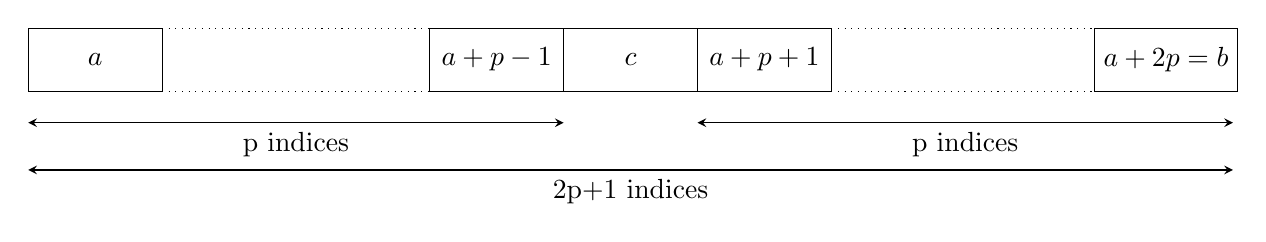
\begin{tikzpicture}[>=stealth]
\tikzstyle{rect}=[rectangle,draw,minimum width =2*\larg,minimum height=2*\haut]
\draw (0,0) node (r1) [rect]{$a$};
\draw[dotted](\larg,-\haut) --(5*\larg,-\haut);
\draw[dotted](\larg,\haut) --(5*\larg,\haut);
\draw (6*\larg,0) node (r2)  [rect]{$a+p-1$};
\draw (8*\larg,0) node (r3)  [rect]{$c$};
\draw (10*\larg,0) node (r4)  [rect]{$a+p+1$};
\draw[dotted](11*\larg,-\haut) --(15*\larg,-\haut);
\draw[dotted](11*\larg,\haut) --(15*\larg,\haut);
\draw (16*\larg,0) node (r4)  [rect]{$a+2p=b$};
\draw [<->](-\larg,-2*\haut) -- node [below] {p indices}  (7*\larg,-2*\haut);
\draw [<->](9*\larg,-2*\haut) -- node [below] {p indices}  (17*\larg,-2*\haut);
\draw [<->](-\larg,-3.5*\haut) -- node [below] {2p+1 indices}  (17*\larg,-3.5*\haut);
\end{tikzpicture}

\medskip
\def\larg{8.5mm}

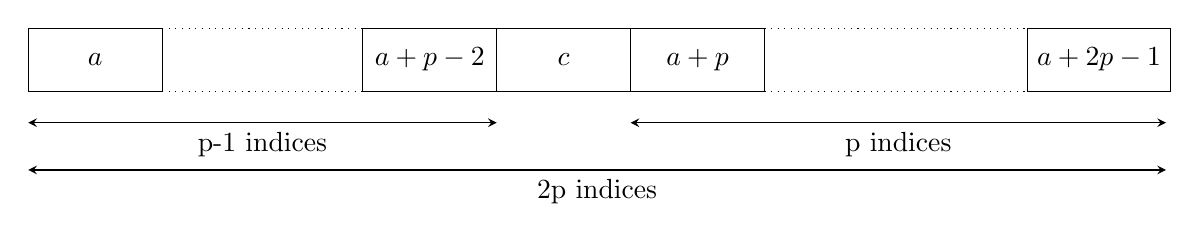
\begin{tikzpicture}[>=stealth]
\tikzstyle{rect}=[rectangle,draw,minimum width =2*\larg,minimum height=2*\haut]
\draw (0,0) node (r1) [rect]{$a$};
\draw[dotted](\larg,-\haut) --(4*\larg,-\haut);
\draw[dotted](\larg,\haut) --(4*\larg,\haut);
\draw (5*\larg,0) node (r2)  [rect]{$a+p-2$};
\draw (7*\larg,0) node (r3)  [rect]{$c$};
\draw (9*\larg,0) node (r4)  [rect]{$a+p$};
\draw[dotted](10*\larg,-\haut) --(14*\larg,-\haut);
\draw[dotted](10*\larg,\haut) --(14*\larg,\haut);
\draw (15*\larg,0) node (r4)  [rect]{$a+2p-1$};
\draw [<->](-\larg,-2*\haut) -- node [below] {p-1 indices}  (6*\larg,-2*\haut);
\draw [<->](8*\larg,-2*\haut) -- node [below] {p indices}  (16*\larg,-2*\haut);
\draw [<->](-\larg,-3.5*\haut) -- node [below] {2p indices}  (16*\larg,-3.5*\haut);
\end{tikzpicture}

On note $\gamma(a,b)$ le nombre de comparaisons nécessaires à l'exécution de \type{chercher\_entre(x, l, a, b)}.

On a ainsi 3 possibilités, en notant \type{m = (a+b)//2}, 
\[ 
\gamma(a, b)= \left\{\begin{matrix} 1\cr  2 + \gamma(a, m-1)\\ 2 + \gamma(m+1, b) \end{matrix}\right.
\]

Si on note $C(k)$ la borne supérieure des complexités pour traiter $k$ indices,  on a donc $C(2p+1) = 2+C(p)$ et $C(2p) = 2 +C(p)$ ; il y a égalité car, dans les deux cas, on peut ne pas trouver l'élément et  aboutir à une liste de taille $p$.

On a $C(0)=0$ d'où $C(1)=2$  puis, par récurrence, $C(2^k) = 2(k+1)$.

\medskip

Prouvons alors que, si $2^{k} \le n < 2^{k+1}$, on a $C(n)=2(k+1)$.
%--------------------------------------------------------------------------
\begin{itemize}
\item Comme on a $C(1)=2$ et $C(2)=4$, le résultat est vrai pour $k=0$ et $k=1$.

\item Si la propriété est vraie pour un entier $k$, on considère $n$ tel que $2^{k+1} \le n \le 2^{k+2}-1$.

\begin{itemize}
\item Si $n$ est pair alors, comme $2^{k+2}-1$ est impair, ces entiers sont distincts donc 

$2^{k+1} \le n =2p \le 2^{k+2}-2$. On a alors $2^{k} \le p \le 2^{k+1}-1$ et l'hypothèse de récurrence donne $C(p)=2(k+1)$ puis $C(n)=C(p)+2=2(k+2)$.

\item Si $n$ est impair alors, comme $2^{k+1}$ est pair, on a $2^{k+1}+1 \le n =2p+1 \le 2^{k+2}-1$ d'où  $2^{k+1} \le  2p \le 2^{k+2}-2$ puis $2^{k} \le p \le 2^{k+1}$. L'hypothèse de récurrence donne $C(p)=2(k+1)$ puis $C(n)=C(p)+2=2(k+2)$.
\end{itemize}
La propriété est alors vraie pour $k+1$.
\item Ainsi, par récurrence,  la propriété est vraie pour tout $k$.
\end{itemize}
%--------------------------------------------------------------------------
Si on  $2^{k} \le n$ alors $k \le \log_2(n)$ donc la complexité, en nombre de comparaisons, est majorée par $2\log_2(n)+2$, c'est un ${\mathcal O}\bigl(\log_2(n)\bigr)$
%--------------------------------------------------------------------------
\newpage
%--------------------------------------------------------------------------
\section{Avantages et inconvénients}
%--------------------------------------------------------------------------
%--------------------------------------------------------------------------
Les exemples ont permis de mettre en évidence des avantages de la programmation récursive par rapport à la programmation itérative.
%--------------------------------------------------------------------------
\begin{itemize}
\item Le code est facile à écrire et à lire en général.
\item La définition récurrente mathématique trouve immédiatement sa traduction informatique.
\item Pour certaines structures de données, celles qui sont elles-mêmes définies récursivement, la récursivité permet de trouver des algorithmes simples et clairs.
\item Les démonstrations de terminaison, correction et de complexité sont plus simples à écrire.
\end{itemize}
%--------------------------------------------------------------------------
\medskip

Un inconvénient a été entrevu : lors des différents appels à la fonction récursive le langage de programmation doit stocker les valeurs des calculs à faire. Il emploie pour cela une pile mais celle-ci a une taille limitée déterminée à l'avance. Lorsque cette mémoire est saturée le langage renvoie le message d'erreur "{\bf stack overflow}".

\medskip

Il peut apparaître un autre problème lorsqu'on traduit une définition par récurrence : il se peut que l'on multiplie les calculs sans s'en rendre compte.

\subsubsection{Exemple : suite de Fibonacci}

La suite de Fibonacci est définie par $ \left\{\begin{matrix} F_0=0 &\cr  F_1=1 &\cr  F_n = F_{n-1}+F_{n-2}&\hbox{ pour  }n \ge 2\cr \end{matrix}\right.$

La traduction récursive immédiate est  
%--------------------------------------------------------------------------
\begin{lstlisting}
def fibo(n) :
  """Entrée : un entier positif n.
     Sortie : le n-ième nombre de Fibonacci"""
    if n <= 1 :
        return(1)
    else :
        return fibo(n-1)+fibo(n-2) 
\end{lstlisting}
%--------------------------------------------------------------------------
La terminaison et la correction de l'algorithme ne posent pas de problème.

Comptons le nombre d'additions, noté $C(n)$, pour calculer $F_n$.

On a facilement $C(0)=C(1)=0$ et $C(n)=C(n-1)+1+C(n-2)$.

Si on retranche\footnote{L'équation $u_{n+2} = u_{n+1}+u_n$ admet $(-1)$ comme suite constante solution.} $-1$ à $C(n)$ en posant $u_n=C(n)-(-1)$ on obtient $u_0=1$, $u_1=1$ et $u_{n} = C(n-1)+1+C(n-2) +1 =u_{n-1}+u_{n-2}$ donc $(u_n)$ vérifie la même récurrence que $F_n$ avec les valeurs initiales décalées d'où $C(n)=u_n-1=F_{n+1}-1$. On montre classiquement que $\displaystyle F_n = \frac{\alpha^{n+1}-\beta^{n+1}}{\sqrt 5}$ avec  $\displaystyle \alpha = \frac{1+\sqrt 5}2$ et  $\displaystyle \beta = \frac{1-\sqrt 5}2$ d'où   $C(n)={\mathcal O}(\alpha^n)$. 

Cette complexité exponentielle rend impossible le calcul pour $n$ dépassant quelques dizaines.

Par exemple $F_{40}$, que l'on calcule à la main avec 39 additions, engendre $F_{41}-1 \sim  4.10^8$ additions  dans le programme ci-dessus ; le calcul prend 80 secondes sur un ordinateur (en 2016).
\newpage

Que se passe-t-il ? 
Voici les calculs faits pour \type{fibo(6)}
%--------------------------------------------------------------------------
\[
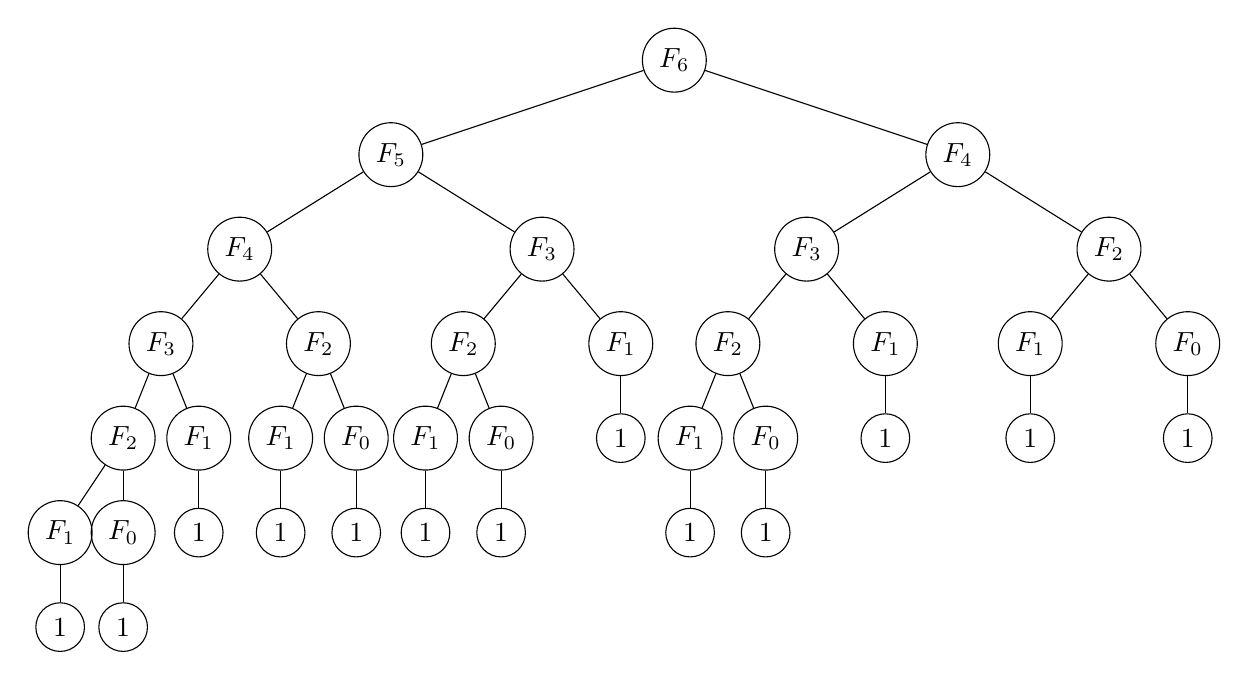
\begin{tikzpicture}[scale=0.8]
  \tikzstyle{level 1}=[sibling distance=90mm]
  \tikzstyle{level 2}=[sibling distance=48mm]
  \tikzstyle{level 3}=[sibling distance=25mm]
  \tikzstyle{level 4}=[sibling distance=12mm]
  \tikzstyle{level 5}=[sibling distance=10mm]
  \tikzstyle{every node}=[circle,draw,minimum size=6mm]
\node{$F_6$}
child{node{$F_5$}
      child{node{$F_4$}
            child {node{$F_3$}
                   child{node{$F_2$}
                         child{node{$F_1$}
                               child{node{$1$}}
                              }
                         child{node{$F_0$}
                               child{node{$1$}}
                              }
                         child[fill=none] {edge from parent[draw=none]}
                        }
                   child{node{$F_1$}
                         child{node{$1$}}
                        }
                  }
            child {node{$F_2$}
                   child{node{$F_1$}
                         child{node{$1$}}
                        }
                   child{node{$F_0$}
                         child{node{$1$}}
                        }
                  }
           }
      child{node{$F_3$}
            child{node{$F_2$}
                  child{node{$F_1$}
                        child{node{$1$}}
                       }
                  child{node{$F_0$}
                        child{node{$1$}}
                       }
                 }
            child{node{$F_1$}
                  child{node{$1$}}
                 }
           }
     }
child{node{$F_4$}
      child {node{$F_3$}
             child{node{$F_2$}
                   child{node{$F_1$}
                         child{node{$1$}}
                        }
                   child{node{$F_0$}
                         child{node{$1$}}
                        }
                  }
             child{node{$F_1$}
                   child{node{$1$}}
                  }
            }
      child {node{$F_2$}
             child{node{$F_1$}
                   child{node{$1$}}
                  }
             child{node{$F_0$}
                   child{node{$1$}}
                  }
            }
     }
 ;
\end{tikzpicture}
\]
%--------------------------------------------------------------------------

On remarque qu'on a fait 5 fois le calcul de $F_2=1+1$ par exemple.

On peut aussi regarder le résultat du programme suivant qui détaille les différents calculs
%--------------------------------------------------------------------------
\begin{lstlisting}
def fiboDecompose(n):
  """Entrée : un entier positif n.
     Sortie : les calculs intermédiaires du calcul
              du n-ième nombre de Fibonacci"""
    print("fibo a ete appele avec n = {}".format(n))
    if n <= 1:
        print('Un cas de base est  atteint')
        return 1
    else:
        res = fiboDecompose(n-1)+fiboDecompose(n-2)
        print('Calcul de F({}) + F({}) = {}'.format(n-1,n-2,res))
\end{lstlisting}
%--------------------------------------------------------------------------

\medskip

Pour parvenir à une complexité raisonnable le plus simple ici est de revenir à un programme itératif.
%--------------------------------------------------------------------------
\begin{lstlisting}
def fibo(n):
  """Entrée : un entier positif n.
     Sortie : le n-ième nombre de Fibonacci"""
    terme=1   # On initialise le premier terme
    suivant=1 # Et le suivant
    for k in range(n):
        precedent = terme
        terme = suivant
        suivant = terme + precedent
    return terme
\end{lstlisting}
%--------------------------------------------------------------------------
On pouvait utiliser le raccourci Python dans la boucle :
%--------------------------------------------------------------------------
\begin{lstlisting}
    for k in range(n):
        terme, suivant = suivant, terme + suivant
\end{lstlisting}
%--------------------------------------------------------------------------
%--------------------------------------------------------------------------
%--------------------------------------------------------------------------
\section{Écriture récursive des tris}
%--------------------------------------------------------------------------
%-------------------------------------------------------------------------------
%--------------------------------------------------------------------------
Les tris étudiés dans le chapitre précédent peuvent être écrits de manière récursive.

Un guide pour écrire les algorithmes est de partir des invariants de boucle.
%--------------------------------------------------------------------------
%--------------------------------------------------------------------------
\subsection{Tri par insertion}
%--------------------------------------------------------------------------
%-------------------------------------------------------------------------------
Pour le tri par insertion un invariant de boucle est que, pour chaque $i$, la liste des $i$ premiers termes est le tri des premiers termes de la liste initiale, le reste étant inchangé.

On peut donc écrire une fonction récursive qui trie les $i$ premiers termes.
\begin{enumerate}
\item il n'y a rien à faire si $i=0$,
\item pour $i\ge 1$, on appelle la fonction avec $i-1$ puis on insère l'élément d'indice $i$
\end{enumerate}
%-------------------------------------------------------------------------------
\begin{lstlisting}
def triPartiel(liste, i):
    """Entrées : une liste et un indice
       Requis  : 0 <= i < len(liste)
       Sortie  : les i premiers éléments sont triés, en place
                 les autres sont inchangés"""
    if i > 0:
        triPartiel(liste, i-1)
        inserer(liste, i-1)
\end{lstlisting}

\begin{lstlisting}
def tri(liste):
    """Entrée : une liste 
       Sortie : la liste est triée"""
    n = len(liste)
    triPartiel(liste, n)
\end{lstlisting}
%--------------------------------------------------------------------------
%--------------------------------------------------------------------------
\subsection{Tri par sélection}
%--------------------------------------------------------------------------
%-------------------------------------------------------------------------------
Pour le tri par sélection, un invariant de boucle est que, pour chaque $i$, les $i$ premiers termes sont les $i$ plus petits termes de la liste.
%-------------------------------------------------------------------------------
\begin{lstlisting}
def triPremiers(liste, i):
    """Entrées : une liste et un indice
       Requis  : 0 <= i < len(liste)
       Sortie  : les i plus petits éléments sont triés"""
    if i > 0:
        triPremiers(liste, i-1)
        k = indMinDepuis(liste, i-1)
        echange(liste, k, i-1)
\end{lstlisting}

\begin{lstlisting}
def tri(liste):
    """Entrée : une liste 
       Sortie : la liste est triée"""
    n = len(liste)
    triPremiers(liste, n)
\end{lstlisting}
%-------------------------------------------------------------------------------
\newpage
%--------------------------------------------------------------------------
%--------------------------------------------------------------------------
\section{Exercices}
%--------------------------------------------------------------------------
%-------------------------------------------------------------------------------
%-------------------------------------------------------------------------------
\begin{Exercise}[title = {Somme de liste}]
Donner un algorithme récursif de calcul de la somme des termes d'une liste qui soit de complexité linéaire.
\end{Exercise}
%--------------------------------------------------------------------------
\begin{Answer}
\begin{enumerate}
\item Ici le problème est de ne pas copier la liste ; il faut donc considérer la liste comme globale. Dans ce cas elle ne peut pas être paramètre de la fonction récursive. On va donc définir une fonction auxiliaire récursive dans laquelle on ajoute l'indice de fin de calcul comme paramètre.
%--------------------------------------------------------------------------
\begin{lstlisting}
def sommeJusquA(liste, k):
    """Entrées : une liste de nombres, un entier
       Requis  : 0 <= k <= len(liste)
       Sortie : la somme des k premiers termes de la liste"""
    if k == 0:
        return 0
    else:
        return  liste[k-1] + sommeJusquA(liste, k-1)

def somme(liste):
    """Entrée : une liste de nombres
       Sortie : la somme des termes de la liste"""
    n = len(liste)
    return sommeJusquA(liste, n)
\end{lstlisting}
%--------------------------------------------------------------------------
\item On pouvait aussi inclure cette fonction auxiliaire {\bf dans} la fonction principale, on n'a plus besoin de donner la liste comme paramètre car elle est une variable globale.
%--------------------------------------------------------------------------
\begin{lstlisting}
def somme(liste):
    """Entrée : une liste de nombres
       Sortie : la somme des termes de la liste"""
    n = len(liste)
    def sommeJusquA(k):
        if k == 0:
            return 0
        else:
            return  liste[k-1] + sommeJusquA(k-1)
    return sommeJusquA(n)
\end{lstlisting}
%--------------------------------------------------------------------------
\item Il existe une construction (spécifique à python) qui permet de se passer d'une fonction auxiliaire. On introduit une variable optionnelle dont la valeur par défaut (ici $-1$) déclenche l'appel avec la valeur adéquate.
%--------------------------------------------------------------------------
\begin{lstlisting}
def somme(liste, long = -1):
    """Entrée : une liste de nombres
       Sortie : la somme des termes de la liste"""
    if longueur == -1:
        return somme(liste, len(liste))
    elif longueur == 0:
        return  0
    else:
        return  liste[-1] + somme(liste, longueur - 1)
\end{lstlisting}
%-------------------------------------------------------------------------------
\newpage
\item On pouvait aussi séparer la liste rapidement avec la méthode \type{pop}. Cependant cela modifie la liste initiale : il faut donc travailler sur une copie.
%--------------------------------------------------------------------------
\begin{lstlisting}
def somme(liste, longueur = -1):
    """Entrée : une liste de nombres
       Sortie : la somme des termes de la liste"""
    liste1 = copie(liste) # à définir, par ex. copy.deepcopy
    def sommeRec(l):
        if l == []:
            return 0
        else:
            x = l.pop()
            return x + sommeRec(l)
    return sommeRec(liste1)
\end{lstlisting}
%--------------------------------------------------------------------------
Un exemple de copie.
%--------------------------------------------------------------------------
\begin{lstlisting}
def copie(liste):
    return [x for x in liste]
\end{lstlisting}
%-------------------------------------------------------------------------------
\end{enumerate}
\end{Answer}
%-------------------------------------------------------------------------------%--------------------------------------------------------------------------
\begin{Exercise}[title = {Suites}]
Écrire en Python une fonction récursive qui calcule le terme d'indice $n$ de la suite $(u_n)$ dans les cas suivants. On précisera le cas de base et la récurrence.
\begin{enumerate}
\item La suite arithmétique  de premier terme 1 et de raison $7$.

\item La suite géométrique de premier terme 1 et de raison $\sqrt{2}$

\item $u_0=2$ et, pour $n\ge  1$, $u_n=4u_{n-1}-1$.

\item $u_{1}=4$ et, pour $n\ge 2$,  $u_{n}=\sqrt{n+u_{n-1}}$.

\item $u_0=1$ et, pour $n\ge  1$, $\displaystyle u_n=\frac12 \left(u_{n-1}+\frac2{u_{n-1}}\right)$.
\end{enumerate}
\end{Exercise}
%--------------------------------------------------------------------------
\begin{Answer}
\begin{enumerate}
\item 
\begin{lstlisting}
def u(n):
    if n == 0:
        return 1
    else:
        return 7 + u (n-1)
\end{lstlisting} 
%-------------------------------------------------------------------------------

\item  
\begin{lstlisting}
def u(n):
    if n == 0:
        return 1
    else:
        return 2**0.5*u (n-1)
\end{lstlisting}
%-------------------------------------------------------------------------------

\item 
\begin{lstlisting}
def u(n):
    if n == 0:
        return 2
    else:
        return 4*u (n-1)-1
\end{lstlisting}
%-------------------------------------------------------------------------------

\item 
\begin{lstlisting}
def u(n):
    if n <= 1:
        return 4
    else:
        return (n+u(n-1))**0.5
\end{lstlisting}
%-------------------------------------------------------------------------------

\item 
\begin{lstlisting}
def u(n):
    if n <= 0:
        return 4
    else:
        v = u(n-1) # Ne pas demander 2 fois le même calcul
        return (v + 2/v)/2
\end{lstlisting}
\end{enumerate}
\end{Answer}
%-------------------------------------------------------------------------------
%-------------------------------------------------------------------------------
\begin{Exercise}[title = {Logarithme entier}]

Le logarithme entier (ou discret) d'un entier $n\ge 1$ est l'entier $p$ tel que 
$2^p \le n < 2^{p+1}$.

Écrire une fonction récursive \type{logEntier(n)} qui le calcule.
\end{Exercise}
%--------------------------------------------------------------------------
\begin{Answer}

Si on a $2^p \le n < 2^{p+1}$ avec $p\ge 1$ alors on a $2^{p-1} \le n//2 < 2^p$.

On peut donc déduire la valeur du logarithme discret de $n$ à partir de celui de $n//2$.

Le cas d'arrêt est 1.

\begin{lstlisting}
def logEntier(n)
    if n==1:
        return 0
    else:
        return 1 + logEntier(n//2)
\end{lstlisting}
\end{Answer}
%-------------------------------------------------------------------------------
%-------------------------------------------------------------------------------
\begin{Exercise}[title = {Coefficients binomiaux}]
À l'aide de la relation $\binom{n}{p}=\binom{n-1}{p}+\binom{n-1}{p-1},$ écrire en Python une fonction récursive  \type{binomAdd(n,p)} qui renvoie la valeur de $\binom{n}{p}$.

On donnera la complexité temporelle en fonction de  $n$.

Si cette complexité n'est pas raisonnable, proposer une amélioration.
\end{Exercise}
%--------------------------------------------------------------------------
\begin{Answer}

Si on applique la définition on peut écrire
\begin{lstlisting}
def binomAdd(n,p):
    if p < 0 or n < p:
        return 0
    elif p == 0 or p == n:
        return 1
    else:        
        return binomAdd(n-1,p-1) + binomAdd(n-1,p)
\end{lstlisting} 

Le programme termine car la valeur de $n$ diminue de 1 à chaque appel.

Si on note $C(n,p)$ le nombre d'additions pour calculer \type{binomAdd(n,p)} on a 

$C(n,n)=C(n,0)=0$ et $C(n,p)=C(n-1,p-1)+C(n-1,p)+1$.

On remarque que si on pose $C'(n,p) = C(n,p)+1$ alors $C'(n,n)=C'(n,0)=1$ 

$C'(n,p)=C'(n-1,p-1)+C'(n-1,p)$ : on a donc $C'(n,p)=\binom{n}{p}$.

Pour $p$ fixé on a ainsi $C(n,p)=\binom{n}{p}-1 = {\cal O}(n^p)$ ce qui est peu efficace. 

Par exemple \type{binomAdd(30,10)} demande 20 secondes de calcul.

\medskip

Pour retrouver une complexité raisonnable il faut éviter de calculer plusieurs fois les mêmes résultats ; la fonction ci-dessus tombe dans ce piège. 

On peut calculer la suite des $\binom mq$ pour $q$ variant de 0 à $m$ pour chaque $m$ de 0 à $n$.
%-------------------------------------------------------------------------------
\begin{lstlisting}
def suiteBinom(n,p):
    if n == 0:
        return [1]
    else:        
        prec = suiteBinom(n-1)
        liste = [1] 
        for i in range(1,n):
            liste.append(prec[k-1]+prec[k])
        liste.append(1)
        return liste
\end{lstlisting} 
%-------------------------------------------------------------------------------
\begin{lstlisting}
def binomAdd1(n,p):
    return suiteBinom(n,p)[p]
\end{lstlisting} 

La complexité est majorée par $np$. \type{binomAdd1(30,10)} est immédiat ($2.10^{-4}$ s, \type{binomAdd1(300,100)} demande 12 ms.
\end{Answer}
%-------------------------------------------------------------------------------
%-------------------------------------------------------------------------------
\begin{Exercise}[title = Exponentiation]

\begin{enumerate}
  \item Que calcule \type{mystere(a,n)} pour $a$ réel $a$ et $n$ entier naturel ?
\begin{lstlisting}
def mystere(a,n):
    """Entrée : un réel a et un entier positif n
       Sortie : ???"""
    if n==0:
        return 1
    else:
        return a*mystere(a,n-1)
\end{lstlisting}
 \medskip
 
\item Pour $k\in\N^* $ on remarque qu'on a $a^{2k}=(a^k)^2$ et $a^{2k+1}=(a^k)^2.a$. 

Utiliser ce résultat pour écrire une fonction récursive \type{puissance(a,n)} qui retourne $a^n$ ($a$ réel et $n$ entier naturel). 
Combien de multiplications sont effectuées ?
\end{enumerate}
\end{Exercise}
%--------------------------------------------------------------------------
\begin{Answer}
\begin{enumerate}
\item La fonction calcule $a^n$.
%--------------------------------------------------------------------------
\item On utilise 2 fois $a^k$, cependant il ne faut le calculer qu'une fois : on place sa valeur dans une variable. 
%--------------------------------------------------------------------------
\begin{lstlisting}
def puissance(a,n):
    """Entrée : un réel a et un entier positif n
       Sortie : a à la puissance n"""
    if n==0:
        return 1
    else:
        b = puissance(a, n//2)
        if n%2 == 0:
            return b*b
        else:
            return b*b*a
\end{lstlisting} 
%--------------------------------------------------------------------------
Si on note $C(n)$ le nombre de multiplication on a $C(n)=C(n//2) +1$ ou $C(n)=C(n//2) +2$ selon que $n$ est pair ou impair avec $C(0)=0$.

Si on a $2^p \le n < 2^{p+1}$ avec $p\ge 1$ alors on a $2^{p-1} \le n//2 < 2^p$.

On note $C'(p)$ un majorant de $C(n)$ pour $2^p \le n < 2^{p+1}$ : on voit qu'on peut choisir $C'(p) = 2 + C'(p-1)$. Comme on peut aussi choisir $C'(0)=C(1)=2$ on en déduit, par récurrence, que $C'(p)=2(p+1)$ convient.

Pour $2^p \le n < 2^{p+1}$ on a $p \le \log_2(n)\bigr)$ donc 
$C(n) \le C'(p) =2(p+1)\le 2\bigl(\log_2(n)+1\bigr)$ 

d'où $C(n)$ est un ${\mathcal O}\bigl(\log_2(n)\bigr)$.
\end{enumerate}
\end{Answer}
%-------------------------------------------------------------------------------
%-------------------------------------------------------------------------------
\subsection{Décomposition de Fibonacci}
%--------------------------------------------------------------------------
%--------------------------------------------------------------------------
\begin{Exercise}[title = {Suite}]\it
Écrire une fonction \type{suiteFibo(n)} qui renvoie la liste des nombres de Fibonacci de $F_0$ à $F_n$.
\end{Exercise}
%--------------------------------------------------------------------------
\begin{Answer}
%--------------------------------------------------------------------------
\begin{lstlisting}
def suiteFibo(n):
    if n == 0:
        return [0]
    elif n == 1:
        return [0, 1]
    else:
        resultat = suiteFibo(n-1)
        # la liste est de taille n
        f = resultat[n-1] + resultat[n-2]
        resultat.append(f)
    return resultat
\end{lstlisting}
\end{Answer}
%-------------------------------------------------------------------------------
%-------------------------------------------------------------------------------

\medskip

Une décomposition de Fibonacci d'un entier $n\ge 1$ est une suite $(F_{k_2}, F_{k_2}, \ldots, F_{k_r})$ de nombres de Fibonacci telle que
\[\left\{\begin{matrix} 
k_1 \ge 2\hfill\\
k_{i+1} \ge k_i +2 \hbox{ pour } 1\le i < r\\
n = F_{k_1} +F_{k_2} + \cdots +F_{k_r} \hfill\\
\end{matrix}\right.\]

Par exemple $300 = 1 + 3 + 8 + 55 + 233 = F_2 + F_4 + F_6 + F_{10} + F_{13}$

\medskip

On peut montrer que si $(F_{k_2}, F_{k_2}, \ldots, F_{k_r})$ est une décomposition de Fibonacci de $n$ alors 

$F_{k_r} \le n < F_{k_r+1}$. On en déduit\footnote{Par récurrence sur $n$.} que $n$ admet au plus une décomposition de Fibonacci.
%-------------------------------------------------------------------------------
%-------------------------------------------------------------------------------
\begin{Exercise}[title = {Nombre de Fibonacci précédent}]\it 
Écrire une fonction \type{precFibo(n)} qui renvoie l'unique entier $p\ge 2$ tel que $F_p \le n < F_{p+1}$.
\end{Exercise}
%--------------------------------------------------------------------------
\begin{Answer}
%--------------------------------------------------------------------------
\begin{lstlisting}
def precFibo(n):
    p = 0
    f = 0
    f_suivant = 1
    while f_suivant <= n:
        p = p + 1
        f_vieux = f
        f = f_suivant
        f_suivant = f_vieux + f
    return p
\end{lstlisting}
\newpage
\end{Answer}
%-------------------------------------------------------------------------------
%-------------------------------------------------------------------------------

\medskip

On peut montrer aussi que si $p$ est la valeur de \type{precFibo(n)} alors une suite de Fibonacci de $n$ peut être construite à partir de celle de $n-F_p$ en lui ajoutant $F_p$. 

Ainsi une décomposition de Fibonacci existe toujours.
%-------------------------------------------------------------------------------
%-------------------------------------------------------------------------------
\begin{Exercise}[title = {Calcul de la décomposition}]\it 
Écrire une fonction \type{decFibo(n)} qui renvoie la décomposition d'un entier $n$ sous la forme d'une liste strictement croissante.
\end{Exercise}
%--------------------------------------------------------------------------
\begin{Answer}
\begin{lstlisting}
def decFibo(n):
    if n == 1:
        return [1]
    else:
        p = precFibo(n)
        l = suiteFibo(p)
        f = l[-1]
        dec = decFibo(n-f)
        dec.append(f)
        return dec
\end{lstlisting}
%--------------------------------------------------------------------------
Cet algorithme n'est pas optimal car il calcule la liste des nombres de Fibonacci à chaque fois. Dans le calcul de la décomposition de $F_2+F_4+\cdots+F_{2r} = F_{2r+1} - 1$ on fera donc $3 + 5 + \cdots +{2r-1}=(2r)^2-1$ sommes, la complexité est quadratique en $p$.

Pour faire mieux on peut écrire
%--------------------------------------------------------------------------
\begin{lstlisting}
def decFibo(n):
    p = precFibo(n)
    l = suiteFibo(p)
    k = len(l)
    indice = k - 1
    dec_inverse = []
    while indice > 1:
        f = l[indice]
        if f <= n:
            dec_inverse.append(f)
            n = n - f
        indice = indice - 1
    dec = dec_inverse[ : : -1] # on retourne la liste
    return dec
\end{lstlisting}
%--------------------------------------------------------------------------
Comme les liste sont de taille $p$, complexité est linéaire en $p$.
\end{Answer}
%--------------------------------------------------------------------------
%--------------------------------------------------------------------------
\subsection{Fractales}
%--------------------------------------------------------------------------
%--------------------------------------------------------------------------
La fractale liée à un motif composé de segments adjacents est la courbe obtenue en remplaçant chaque segment par le motif réduit et en recommençant de manière récursive. La fractale mathématique est l'objet limite, nous allons en tracer une approximation en itérant $n$ fois le procédé.

Par exemple si le motif de base de gauche est transformé en la fractale de droite,  appelée parfois "flocon de Von Koch".
%--------------------------------------------------------------------------
\[
\begin{tikzpicture}
\draw (0,0)-- (2,0) -- ++(60:2) -- ++(-60:2) -- ++(2,0);
\end{tikzpicture}
\hskip 1cm
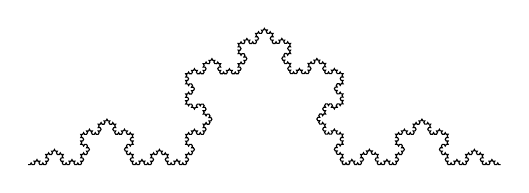
\begin{tikzpicture}[decoration=Koch snowflake]
    \draw decorate{ decorate{ decorate{ decorate{ decorate{ (0,0) -- (6,0) }}}}};
\end{tikzpicture}
\]
%--------------------------------------------------------------------------
Le module \type{turtle} est un ensemble d'outils permettant de dessiner à l'aide d'instructions simples. Ses principales fonctions sont 
%--------------------------------------------------------------------------
\begin{itemize}
\item \type{reset()} : on efface tout et on recommence,
\item \type{goto(x,y)} : aller à l'endroit de coordonnés $x$ et $y$,
\item \type{forward(distance)} : avancer  d'une distance donnée,
\item \type{backward(distance)}  : reculer,: 
\item \type{up()} et \type{down()} : relever et abaisser le crayon,

\item \type{color(couleur)} : Changer de couleur, ('red', 'blue' \dots)
\item \type{left(angle)} et type{right(angle)} : tourner d'un angle donné (en degrés)
\item \type{width(épaisseur)}  : Choisir l'épaisseur du tracé
\item \type{fill(1)} : Remplir un contour fermé à l'aide de la couleur sélectionnée,  

on termine la construction par \type{fill(0)},
\item  \type{write(texte)}  : écrire un texte.
\end{itemize}
%--------------------------------------------------------------------------
Dans l'exemple ci-dessus on remplace un segment de longueur c, \type{forward(c)}; par le programme
%--------------------------------------------------------------------------
\begin{lstlisting}
forward(c/3.0)
left(60)
forward(c/3.0)
right(120) 
forward(c/3.0)
left(60)
forward(c/3.0)
\end{lstlisting}
%-------------------------------------------------------------------------------
%-------------------------------------------------------------------------------
\begin{Exercise}[title = {Tracé}]\it 

Écrire en Python une fonction récursive \type{motif(c,n)} qui trace l'approximation de niveau $n$ de la courbe définie ci-dessus.

Essayer d'autres motifs.
\end{Exercise}
%--------------------------------------------------------------------------
\begin{Answer}

\begin{lstlisting}
def motif(c,n):
    if n==0 :
        forward(c)
    else :
        motif(c/3, n-1)
        left(60)
        motif(c/3, n-1)
        right(120)
        motif(c/3, n-1)
        left(60)
        motif(c/3, n-1)

\end{lstlisting}

\newpage
\end{Answer}
%------------------------------------------------------------
%------------------------------------------------------------




